% *********************************************************************
% © 2010–2022 Jeremy Sylvestre
%
% Permission is granted to copy, distribute and/or modify this document
% under the terms of the GNU Free Documentation License, Version 1.3 or
% any later version published by the Free Software Foundation; with no
% Invariant Sections, no Front-Cover Texts, and no Back-Cover Texts. A
% copy of the license is included in the appendix entitled “GNU Free
% Documentation License” that appears in the output document of this
% PreTeXt source code. All trademarks™ are the registered® marks of
% their respective owners.
%
% *********************************************************************

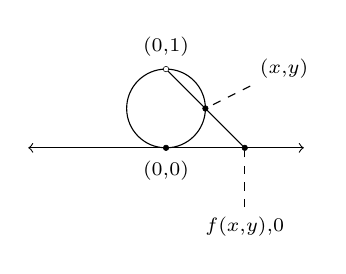
\begin{tikzpicture}[
	vertex/.style={ circle, draw, very thin, fill, inner sep=0pt, minimum size=2pt },
	vertexg/.style={ black!40!white, circle, draw, very thin, fill, inner sep=0pt, minimum size=2pt },
	vertexo/.style={ circle, draw, very thin, inner sep=0pt, minimum size=2pt }
]

\draw (0,0.5) circle (0.5cm);
\fill[white] (0,1) circle (1pt);
\node at (0,1) (np) [vertexo,label=above:{$\scriptstyle (0,1)$}] {};
\node at (0,0) (origin) [vertex,label=below:{$\scriptstyle (0,0)$}] {};
\draw[->] (origin.west) -- (-1.75,0);
\draw[->] (origin.east) -- (1.75,0);
\node[vertex] at (0.5,0.5) (cpt) {};
\node at (1.5,1) (cptlabel) {$\scriptstyle (x,y)$};
\draw[dashed] (cptlabel) -- (cpt);
\node[vertex] at (1,0) (gpt) {};
\node at (1,-1) (gptlabel) {$\scriptstyle \bbrac{f(x,y),0}$};
\draw[dashed] (gptlabel) -- (gpt);
\draw (gpt) -- (np);


\end{tikzpicture}
